% ----------------------------------------------------
% Integration to Wild-Life 
% ----------------------------------------------------
\documentclass[class=report,11pt,crop=false]{standalone}
% Page geometry
\usepackage[a4paper,margin=20mm,top=25mm,bottom=25mm]{geometry}
\usepackage{indentfirst}
% Font choice
\usepackage{lmodern}

% Use IEEE bibliography style
\bibliographystyle{IEEEtran}

% Line spacing
\usepackage{setspace}
\setstretch{1.20}

% Ensure UTF8 encoding
\usepackage[utf8]{inputenc}

% Language standard (not too important)
\usepackage[english]{babel}

% Skip a line in between paragraphs
\usepackage{parskip}

% For the creation of dummy text
\usepackage{blindtext}

% Math
\usepackage{amsmath}

\usepackage{enumitem}


% Header & Footer stuff
\usepackage{fancyhdr}
\pagestyle{fancy}
\fancyhead{}
\fancyhead[R]{\nouppercase{\rightmark}}
\fancyfoot{}
\fancyfoot[C]{\thepage}
\renewcommand{\headrulewidth}{0.0pt}
\renewcommand{\footrulewidth}{0.0pt}
\setlength{\headheight}{13.6pt}

% Epigraphs
\usepackage{epigraph}
\setlength\epigraphrule{0pt}
\setlength{\epigraphwidth}{0.65\textwidth}

% Colour
\usepackage{color}
\usepackage[usenames,dvipsnames]{xcolor}

% Hyperlinks & References
\usepackage{hyperref}
\definecolor{linkColour}{RGB}{77,71,200}%{0,144,208}%
\hypersetup{
    colorlinks=true,
    linkcolor=linkColour,
    filecolor=linkColour,
    urlcolor=linkColour,
    citecolor=linkColour,
}
\urlstyle{same}

% Automatically correct front-side quotes
\usepackage[autostyle=false, style=ukenglish]{csquotes}
\MakeOuterQuote{"}

% Graphics
\usepackage{graphicx}
\graphicspath{{Images/}{../Images/}}
\usepackage{makecell}
\usepackage{transparent}

% SI units
\usepackage{siunitx}

% Microtype goodness
\usepackage{microtype}

% Listings
\usepackage[T1]{fontenc}
\usepackage{listings}
\usepackage[scaled=0.8]{DejaVuSansMono}

% Custom colours for listings
\definecolor{backgroundColour}{RGB}{250,250,250}
\definecolor{commentColour}{RGB}{10, 204, 10}
\definecolor{identifierColour}{RGB}{0, 0, 255}%{196, 19, 66}
\definecolor{stringColour}{RGB}{255, 0, 255}
\definecolor{keywordColour}{RGB}{255,0,0}
\definecolor{lineNumbersColour}{RGB}{127,127,127}
\lstset{
  language=Python,
  captionpos=b,
  aboveskip=10pt,belowskip=10pt,
  backgroundcolor=\color{backgroundColour},
  basicstyle=\ttfamily,%\footnotesize,        % the size of the fonts that are used for the code
  breakatwhitespace=false,         % sets if automatic breaks should only happen at whitespace
  breaklines=true,                 % sets automatic line breaking
  postbreak=\mbox{\textcolor{red}{$\hookrightarrow$}\space},
  commentstyle=\color{commentColour},    % comment style
  identifierstyle=\color{identifierColour},
  stringstyle=\color{stringColour},
   keywordstyle=\color{keywordColour},       % keyword style
  %escapeinside={\%*}{*)},          % if you want to add LaTeX within your code
  extendedchars=true,              % lets you use non-ASCII characters; for 8-bits encodings only, does not work with UTF-8
  frame=single,	                   % adds a frame around the code
  keepspaces=true,                 % keeps spaces in text, useful for keeping indentation of code (possibly needs columns=flexible)
  morekeywords={*,...},            % if you want to add more keywords to the set
  numbers=left,                    % where to put the line-numbers; possible values are (none, left, right)
  numbersep=5pt,                   % how far the line-numbers are from the code
  numberstyle=\tiny\color{lineNumbersColour}, % the style that is used for the line-numbers
  rulecolor=\color{black},         % if not set, the frame-color may be changed on line-breaks within not-black text (e.g. comments (green here))
  showspaces=false,                % show spaces everywhere adding particular underscores; it overrides 'showstringspaces'
  showstringspaces=false,          % underline spaces within strings only
  showtabs=false,                  % show tabs within strings adding particular underscores
  stepnumber=1,                    % the step between two line-numbers. If it's 1, each line will be numbered
  tabsize=2,	                   % sets default tabsize to 2 spaces
  %title=\lstname                   % show the filename of files included with \lstinputlisting; also try caption instead of title
}

% Caption stuff
\usepackage[hypcap=true, justification=centering]{caption}
\usepackage{subcaption}

% Glossary package
% \usepackage[acronym]{glossaries}
\usepackage{glossaries-extra}
\setabbreviationstyle[acronym]{long-short}

% For Proofs & Theorems
\usepackage{amsthm}

% Maths symbols
\usepackage{amssymb}
\usepackage{mathrsfs}
\usepackage{mathtools}

% For algorithms
\usepackage[]{algorithm2e}

% Spacing stuff
\setlength{\abovecaptionskip}{5pt plus 3pt minus 2pt}
\setlength{\belowcaptionskip}{5pt plus 3pt minus 2pt}
\setlength{\textfloatsep}{10pt plus 3pt minus 2pt}
\setlength{\intextsep}{15pt plus 3pt minus 2pt}

% For aligning footnotes at bottom of page, instead of hugging text
\usepackage[bottom]{footmisc}

% Add LoF, Bib, etc. to ToC
\usepackage[nottoc]{tocbibind}

% SI
\usepackage{siunitx}

% For removing some whitespace in Chapter headings etc
\usepackage{etoolbox}
\makeatletter
\patchcmd{\@makechapterhead}{\vspace*{50\p@}}{\vspace*{-10pt}}{}{}%
\patchcmd{\@makeschapterhead}{\vspace*{50\p@}}{\vspace*{-10pt}}{}{}%
\makeatother
\makenoidxglossaries


\newacronym{fm}{FM}{Frequency Modulation}
\newacronym{am}{AM}{Amplitude Modulation}
\newacronym{em}{EM}{electromagnetic}
\newacronym{iq}{IQ}{In-phase and Quadrature}


\newacronym{dft}{DFT}{Discrete Fourier Transform}
\newacronym{idft}{IDFT}{Inverse Discrete Fourier Transform}
\newacronym{fft}{FFT}{Fast Fourier Transform}
\newacronym{ifft}{IFFT}{Inverse Fast Fourier Transform}

\newacronym{df}{DF}{Direction Finding}
\newacronym{rdf}{RDF}{Radio Direction Finding}
\newacronym{AoA}{AoA}{Angle of Arrival}
\newacronym{rf}{RF}{Radio Frequency}
\newacronym{sdr}{SDR}{Software-Defined Radio}
\newacronym{pd}{PD}{Phase-Difference}
\newacronym{vhf}{VHF}{Very High Frequency}
\newacronym{MHz}{MHz}{Megahertz}
\newacronym{db}{dB}{decibel}
\newacronym{dbm}{dBm}{Decibel-milliwatts}
\newacronym{rx}{Rx}{Receiver}
\newacronym{tx}{Tx}{Transmitter}
\newacronym{dsp}{DSP}{Digital Signal Processing}
\newacronym{vor}{VOR}{Very High Frequency Omnidirection Range}
\newacronym{gps}{GPS}{Global Position System}
\newacronym{adf}{ADF}{Automatic Direction Finders}
\newacronym{ndb}{NDB}{Non-Directional Beacon}
\newacronym{sm}{S meter}{Signal Strength Meter}
\newacronym{tdoa}{TDOA}{Time Difference of Arrival}
\newacronym{ham}{HAM}{an informal name for an amateur radio operator}
\newacronym{wbfm}{WBFM}{Wideband Frequency Modulation}
\newacronym{if}{IF}{Intermediate Frequency}
\newacronym{lp}{LP}{Low Pass}
\newacronym{API}{API}{Application Programming Interface}
\newacronym{fpga}{FPGA}{Field-Programmable Gate Array}
\newacronym{bw}{BW}{Bandwidth}
\newacronym{adc}{ADC}{Analog-to-digital converter}
\newacronym{tv}{Tv}{Television}
\newacronym{ai}{AI}{Artificial Intelligence}
\newacronym{lo}{LO}{Local Oscillator}
\newacronym{icasa}{ICASA}{Independent Communications Authority of South Africa}
\newacronym{usb}{USB}{Universal-serial Buss}
\newacronym{os}{OS}{Operating System}
\newacronym{mimo}{MIMO}{Mutliple input, Multiple output}
\newacronym{vna}{VNA}{Vector Network Analyser}
\newacronym{mse}{MSE}{Mean Squared Error}
\newacronym{SNR}{SNR}{Signal-to-Noise Ratio}

\begin{document}
% ----------------------------------------------------
\chapter{Wildlife telemetry application and integration \label{ch:application}}
\epigraph{``Where the waters do agree, it is quite wonderful the relief they give.''}%
    {\emph{---Jane Austen, Emma}}
\vspace{0.5cm}
% ----------------------------------------------------

%---------------------------------
% Overview
%---------------------------------
\section{Overview}
The aim of this brief chapter is to take a step back from the project, and provide an illustrative idea of how the system developed would be integrated into a \emph{fully fledged} \gls{df} system. This project focused on the validation that through Phase Interferometry, and thus \gls{pd}, \gls{df} is possible on a \gls{sdr} device. This chapter provides the broader motivation for the project, which the limited scope, unfortunately, did not allow for. While a working \gls{df} prototype was developed, the system was not optimised fully to allow for such an integration. The work done is this chapter is purely for the benefit of the reader, to illustrate an integration of this project.


%---------------------------------
% System Descritpion
%---------------------------------
\section{System Description}
The following is a system description for typical use in wildlife telemetry, within the context of African animals and the available products.


A list of considerations for the \gls{sdr} based of parameters from the collar as a transmitter:


\begin{minipage}[t]{.5\linewidth}\centering
\begin{center}
    \begin{tabular}{c}
        \textbf{Requirements} \\
        \hline
        Center frequency = 150MHz \\
        Pulse rate = 1100MS \\
        Pulse width = 20MS \\
        Calibration tolerance = $\pm$2.5kHz \\
        Sampling frequency = 20MSps \\
        Sampling window = 1200MS \\
        Battery life - up to three years \\
    \end{tabular}
\end{center}
\end{minipage}%
\hspace{0.5cm}
\begin{minipage}[t]{.5\linewidth}\centering
\begin{center}
    \begin{tabular}{c}
        \textbf{Base Station}  \\
        \hline
        Minimum three antenna \\
        Battery backup \\
        Local web-serve on host Pi \\
        Weather proof \\
        touchscreen interface \\
        Low powered mode \\
        Real-time clock \\
    \end{tabular}
\end{center}
\end{minipage}

%---------------------------------
% System Triangulation
%---------------------------------
\section{Triangulation}
It has already been discussed that using at least three antenna in the array resolves ambiguities of angles and thus the \gls{df} system is capable of producing a 360-degree bearing \gls{AoA}.

In order to calculate the exact bearing angle from a base station, the same methodology used in this report can be used with some further extension. The calculated \gls{AoA} produced in this report represents a symmetrical angle pair, \emph{in other words} it is not known whether this incident \gls{AoA} is coming from in front of or behind the device. However, if two antennae are used to produce a pair of \gls{AoA} and then within the same antenna array any other combination of two antennae separately produces another two \gls{AoA} possibilities, there will be a common \gls{AoA} between the four \gls{AoA} results. This is then the resolved, true \gls{AoA} in a 360-degree bearing. 

If a system is implemented in which two separated \gls{df} system base stations are producing 360-degree bearing angles and the line produced by the produced \gls{AoA} is plotted, then the intersection of the two lines is calculated, then triangulation is possible. The result is then the exact coordinates of a collar if overlaid onto a map of the farm per say as represented in Figure \ref{fig:wildlife-trian-a}

\begin{figure}[h]\centering
    \subfloat[DF Triangulation possible with two base stations, each consisting with 3 antenna]{\label{fig:wildlife-trian-a}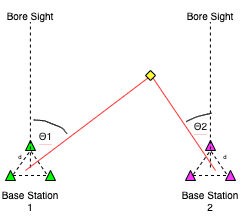
\includegraphics[width=.4\linewidth]{Images/diagrams/wildlife-triangulation.png}}\hspace{0.5cm}
    \subfloat[Calculation of gradient of a line via inclination angle]{\label{fig:wildlife-trian-b}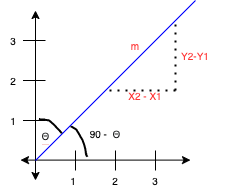
\includegraphics[width=.4\linewidth]{Images/diagrams/Wildlife-gradient.png}}\hfill 
    \caption{Multiple base station geometry used to triangulate a signal source using phase interferometery}
    \label{fig:wildlife-trian}
\end{figure}


From the angle calculated via phase interferometry of each base station $\theta1$ and $\theta2$, the gradient of the euclidean line that this angle produces can be deduced as shown in Figure \ref{fig:wildlife-trian-b}. Mathematically speaking:

\begin{equation*}
\begin{split}
    m = \frac{\Delta y}{\Delta x} \\
    \tan \theta = \frac{\Delta y}{\Delta x} \\
    \therefore m = \tan(90 - \theta) 
\end{split}
\end{equation*}

\newpage
And a briefly, using the equation of two lines: $L_1$ and $L_2$, the point of intersection $(h,k)$ can be calculated:
\begin{equation*}
    \begin{split}
        L_1 : y-y_1 = m_1 (x-x_1) \\
        L_2 : y-y_2 = m_2 (x-x_2) \\
    \end{split}
\end{equation*}
Where $(x_1,y_1)$ and $(x_2,y_2)$ are the know coordinates of the base station, from which the inclination line originates. 

To find $x$ intersection of $L_1$ and $L_2$ lines at $h$, setting $L_1 = L_2$:
\begin{equation*}
    \begin{split}
        m_1(h-x_1) + y_1 = m_2(h-x_2) + y_2 \\
        \therefore h = \frac{(m_2 x_2 - m_1 x_1) - (y_2 - y_1)}{m_2 - m_2}
    \end{split}
\end{equation*}

*Note, $k$ can now be found by substituting into $h = x$ into $L_1$ equation. 


%---------------------------------
% System Descritpion
%---------------------------------
\section{System Display}
An example of the system display used to interface with the two base-station \gls{sdr}.
\begin{figure}[h]
    \centering
    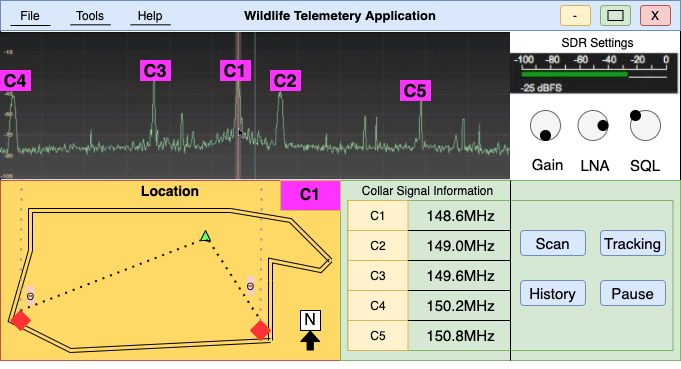
\includegraphics[width=0.9\textwidth]{Images/diagrams/WLT Display.drawio.png}
    \caption{Illustration of Wildlife telemetry application display}
    \label{fig:application-display}
\end{figure}


This brief chapter aimed to provide a general overview on how a \gls{df} system using this project may be extended for use in a wildlife telemetry application. Additionally, some of the future considerations needed for this extension were mentioned.  This will be built on further in Chapter~\ref{ch:fw}. This however clearly shows the scope for further development and the envisioned real-world application. 

% ----------------------------------------------------
\ifstandalone
%\bibliography{Bibliography/References.bib}
\printnoidxglossary[type=\acronymtype,nonumberlist]
\fi
\end{document}
is% ----------------------------------------------------